%!TEX root = ../../Heun_Dale_Haney_A_dynamic_approach_to_input_output_modeling.tex
%%%%%%%%%%%%%%%%%%%%% chapter.tex %%%%%%%%%%%%%%%%%%%%%%%%%%%%%%%%%
%
% sample chapter
%
% Use this file as a template for your own input.
%
%%%%%%%%%%%%%%%%%%%%%%%% Springer-Verlag %%%%%%%%%%%%%%%%%%%%%%%%%%
%\motto{Use the template \emph{chapter.tex} to style the various elements of your chapter content.}
\motto{Where there is no reliable accounting 
and therefore no competent knowledge
of the economic and ecological effects of our lives,
we cannot live lives that are economically
and ecologically responsible. 
It is futile to plead and protest and lobby 
in favor of public ecological responsibility while, 
in virtually every act of our private lives, 
we endorse and support an economic system 
that is by intention, 
and perhaps by necessity, 
ecologically irresponsible.\emph{\cite[p.~26]{Berry1998}}

\hfill---\emph{Wendell Berry}}


%%%%%%%%%%%%%%%%%%%%%%%%%%%%%%%%%%
%%%%%%%%%% Introduction %%%%%%%%%%
%%%%%%%%%%%%%%%%%%%%%%%%%%%%%%%%%%
\chapter{Introduction}
% Always give a unique label
\label{chap:intro}
% use \chaptermark{}
% to alter or adjust the chapter heading in the running head
\chaptermark{Introduction}
%%%%%%%%%%%%%%%%%%%%%%%%%%%%%%%%%%
%%%%%%%%%%%%%%%%%%%%%%%%%%%%%%%%%%
%%%%%%%%%%%%%%%%%%%%%%%%%%%%%%%%%%


%% \abstract{Each chapter should be preceded by an abstract (10--15 lines long) that summarizes the content. The abstract will appear \textit{online} at \url{www.SpringerLink.com} and be available with unrestricted access. This allows unregistered users to read the abstract as a teaser for the complete chapter. As a general rule the abstracts will not appear in the printed version of your book unless it is the style of your particular book or that of the series to which your book belongs.\newline\indent
%% Please use the 'starred' version of the new Springer \texttt{abstract} command for typesetting the text of the online abstracts (cf. source file of this chapter template \texttt{abstract}) and include them with the source files of your manuscript. Use the plain \texttt{abstract} command if the abstract is also to appear in the printed version of the book.}

%% Use the template \emph{chapter.tex} together with the Springer document class SVMono (monograph-type books) or SVMult (edited books) to style the various elements of your chapter content in the Springer layout.

\abstract*{**** Re-write the abstract. ****
In this chapter we give our motivation for writing this book. 
We outline some of the models and subsequent metaphors 
that have been used to describe the economy---clockwork, 
machine, engine---and suggest a new metaphor---the 
metabolism of an organism.
We give an overview of Leontief input-output methods
and their extension to include energy and material inputs
and waste flows out of the economy.
We then propose a new input-output analysis method,
fitting to the new metaphor of the metabolic economy;
a dynamic accounting framework that includes accumulation of stocks
within economic sectors.}

****	Red queen \& treadmill of production





\begin{quote}
by year 50 the cost of maintaining the capital stock 
has overwhelmed the income from resource extraction, 
so profits are no longer sufficient to keep investment ahead of depreciation. 
The operation quickly shuts down, as the capital stock declines. 
The last and most expensive of the resource stays in the ground; 
it doesn't pay to get it out~\cite[p.60]{Meadows2008}
\end{quote}
****

This book is primarily about accounting and change.
It is borne out of a belief that our economies are in constant flux;
changing dynamically in the short-term with human behavior
and evolving over longer time frames 
in response to technological change and
external pressures.
Real-world systems, including economies, are messy and chaotic.
They do not march orderly from one state to the next.

This is also a book about metaphors and models.
We use metaphors to simplify and make sense of the world around us.
They influence us as stories we tell ourselves.
These metaphors inform the mental and empirical models we construct.
And, as we collect data (via accounting methods) 
to assess the validity of those models,
our perception of the world is molded and shaped
by our accounting, which was initially informed
by the stories we told ourselves about reality.
Our models tell us what aspects of the world
are important to value 
(in the literal sense of making measurements),
and also, by extension, 
which parts of the world (literally) have no value.
This process has a deeper normative
consequence: the aspects of the world to which our models ascribe
value are \emph{valuable},
and those ascribed no value become \emph{worthless}.


%%%%%%%%%% Limits %%%%%%%%%%
\section{Limits: Extraction, substitution, and assimlation}
\label{sec:limits}
%%%%%%%%%%

The Preface demonstrates that, at least in the U.S., 
we are not accounting for natural assets, 
including the important categories of materials and energy,
in a way that informs meaningful economic discussion or
leads to enlightened natural resource and energy policies.
Whether you think this is a problem depends, in part, on 
whether you think the world's economies are approaching 
	natural resource extraction limits;
whether you think the materials and energy upon which our economies currently depend
	can be easily substituted by other, readily-available, inexpensive resources; and
whether you think that the world's economies have exceeded 
	the biosphere's waste assimilation capacity.


%+++++++++ Scarcity ++++++++++
\subsection{Natural resource extraction limits}
\label{sub:natural_resource_extraction_limits}
%+++++++++

For many commodities, supply is scarce relative to demand, 
with oil providing, arguably, the most important example. 
Both economic and physical arguments can be used to show that the world is facing
natural resource extraction limits.

Economic theory predicts that as demand for a product, such as oil, increases,
the increased profitability will induce current producers to increase supply, 
additional producers to enter the market,
or other producers to offer close substitutes. 
In the case of natural resources, if that does not happen
then there is evidence that resource extraction limits are being reached.
This is true in the case of oil.
For much of the twentieth century, the price of oil remained below \$20 per barrel.
However, in the 2001--2008 timeframe,
the inflation-adjusted price of oil increased 260\%,
from around \$35 to a peak of \$126 per barrel 
(in constant 2010 USD).
During the same period,
world oil production rose from 
78~million barrels per day to 86~million barrels per day,
an increase of only 10\%.\cite{EIA2014}
Since 2010, the price of oil has remained above \$80 per barrel,
suggesting that production cannot increase quickly enough to bring prices
back down to historical levels.
Persistently high prices for such an important commodity
suggest very real limits to production, 
that supply is constrained relative to demand. 
We have reached natural resource extraction limits.

On a physical basis, 
it is evident that easiest-to-reach resources are extracted first. 
After the easiest-to-reach resources are depleted (such as oil in West Texas),
difficult-to-extract resources are exploited
further offshore,
in harsher environments, and
with enhanced techniques (such as steamflooding or hydraulic fracturing).
Sometimes, new, energy-intensive techniques are required 
for difficult deposits, such as oil sands.
Turning to materials extraction, the production of finer-grade ores
requires the processing of greater amounts of raw material, 
resulting in increasing tailings.
The processing of extra raw material takes more energy, and 
the energetic cost of extracting many materials is certainly increasing.\cite{Hall1986, Mudd2010,Hall2011}
This process has been labeled the ``Red Queen'' effect, 
where we must develop more and more resources to achieve the same
level of production---run faster and faster to stay in 
the same place.\cite{Lees1975, Ross1988, Murray2013, Murphy2014}
% *** BRH says: Isn't this a good place to cite Hall, too? ***
The facts that (a) producers continue to reach deeper and farther 
and (b) energetic costs of production continue to rise
are further evidence that the world is reaching natural resource extraction limits.


%+++++++++ Substituion ++++++++++
\subsection{Substitutability of natural resources}
%+++++++++

The ability to substitute human-made capital for natural resources
or one natural resource for another 
may alleviate the problem of natural resource scarcity relative to demand,
at least temporarily.
There are many historical cases of this sort of substitution occurring,
particularly in the energy sector.
Biomass, mostly wood,
formed the energetic foundation of pre-industrial society.
Deforestation within Europe,
primarily for fuel to smelt iron,~\cite{Smil1994}
prompted the switch to coal.
Whale oil was replaced by petroleum-based kerosene for lighting.\cite{Weissenbacher2009}
Natural gas has begun to replace oil in many applications.
Therefore, goes the argument, 
substitution may continually stave off resource scarcity.

Unfortunately, there are technical limits to this sort of substitution.
For example, there are no known substitutes for oil 
in many sectors of the economy.\cite{Hirsch2005}
Bio-fuels were hailed by many as a viable alternative,
but there is not enough land for bio-fuels to meet demand.
The U.S.\ obtains 13 billion gallons of bio-ethanol 
(less than 10\% of the 134 billion gallons of fuel consumed in 2012)
by diverting approximately 40\%
of domestic corn production.\cite{EIA2014, USDA2014}
**** Discuss the lack of substitutibility **** 
**** Refer to deWit and Heun thinkpiece ****
**** Refer to Stern, Pelli, the Italian author on (lack of) 
substitutability of renewables for FFs. ****

Often, the substitution of man-made resources for natural resources
requires the use of greater amounts of energy.
For example, the production of fresh water from recycled or sea-water
can be particularly energy intensive.
Thus the substitution of one natural resource (fresh water)
for a manufactured resource (desalinated water)
required greater inputs of natural resources (free energy) to achieve.
Free energy is the ultimate natural resource, because energy cannot be 100\% recycled,
whereas material resources can \emph{theoretically} be recycled indefinitely.


%+++++++++ Overloading assimilation capacity ++++++++++
\subsection{Overloading the biosphere's assimilative capacity}
%+++++++++

There are multiple examples of society exceeding 
the assimilative capacity of the biosphere, locally.
In 1952, London city experienced a lethal smog cloud,
due to coal-burning power stations,
that, according to some, claimed up to 12,000 lives.\cite{Davis2002,Bell2004}
China is currently experiencing similar problems.
Such localized environmental problems can often be overcome. 
However,
there are many pollutants that are emitted in multiple localities,
or that, especially in the case of air-pollution, have non-local effects.
%**** Mik: Provide some systemic examples here. ****
Such pollution includes:
algal blooms and so-called ``dead zones'' due to over-use of agricultural fertilizers;
over-use of agricultural pesticides;
build-up of persistent organic pollutants, especially endocrine disruptors, such as PCBs 
and BPAs;\footnote{Polychlorinated biphenyl (PCB) is a synthetic organic chemical often used as 
	a dielectric or coolant in electrical equipment, which is a know carcinogen.
	Bisphenol (BP) A is a carbon-based synthetic compound used in the production
	of plastics and epoxy resins. It exhibits hormone-like properties at high doses.}
bio-accumulation of heavy metals released due to mineral extraction and industrial processing;
ozone depletion due to release of chlorinated gases (primarily halocarbons);
acid rain due to release of sulphur dioxides;
release of radioactive materials;
detergents in sewage;
invasive species;
oil spills;
and, of course, the potential impacts of increased global temperatures 
due to climate change.\cite{Butler1978, UNMEA2005, Walker2012}


\subsection{Disruption of ecosystem function}


There is mounting evidence of more systemic
damage occurring due to society's increasing pressure on
the biosphere.\cite{MEA2005,Ewing2008}
In the drive to reduce costs and increase profits,
natural systems often bear the externalized costs
of increasing production.\footnote{Of course,
	the perspective of external and internal is subjective.
	From the point-of-view of some members of society
	the costs have been externalized, 
	that is they no longer bear the full cost of production;
	those costs have been shared about.}
So-called `free' natural resources are exploited,
land-use is altered to better suit societies needs
and other species are marginalized by the encroach of human activity.\cite{Schnaiberg1980}
In many cases, as more waste is deposited into ecosystems
and as their structures are changed by human activity,
the assimilative capacity of ecosystems declines.\cite{UNMEA2005}
**** MCD - not sure if this belongs here ****
Schnaiberg (1980) introduced the concept of 
the ``treadmill of production'' to describe the systemic process of
increasing capital investment inherent in capitalist society
leading to ``higher and higher levels of demand for natural resources 
for a given level of social welfare''.\cite[p.297]{Gould2004}
The logic of the treadmill runs such that:
\begin{enumerate}
	\item more capital was becoming accumulated in Western economies, and 
	\item this capital was being applied to replacing production labor 
				with new technologies to increase profits; 
	\item these new technologies required far more energy and/or chemicals 
				to replace previous, labor-intensive processes;
	\item new technologies emerged from the organization of scientific and 
				technological research in universities and research institutes, 
				as well as in the new ``research and development'' departments of large firms;
	\item moreover, unlike the prior use of labor, the new technologies represented forms of sunk capital. 
	\item to further increase profits, managers of firms needed to increase the levels of production 
				and sustain higher levels (because worker inputs could more readily be cut back 
				as opposed to fixed costs of machine operations).\cite[p.296]{Gould2004}
\end{enumerate}

%Logic of the treadmill:
%
%\begin{enumerate}
%	\item{increasing accumulation of wealth, through ownership of economic organizations that successfully
%				use ecological resources to expand production and profits;}
%	\item{increasing movement of workers from self-employment, into positions of employees 
%				who must rely on expanded production to gain jobs and wages;}
%	\item{increasing allocations of the accumulated wealth to newer technologies
%				in order to replace labor with physical capital,
%				thereby generating more profits for wealth-holders,
%				in order to sustain and expand their ownership in the face of
%				growing competition from other wealth-holders;}
%	\item{increasing activities of governments to facilitate expanded 
%				accumulation of wealth for ``national development,''
%				on the one hand, and ``social security,''
%				on the other;}
%	\item{the net result of these processes is an increasing necessity for ever greater
%				ecological withdrawals and additions in order to sustain a given level of
%				social welfare;}
%	\item{the ecological obverse of point 5. is the increasing likelihood of an
%				industrial society creating \emph{ecological} disorganization,
%				as economic pressures push toward greater extraction of market values
%				from ecosystems;}
%	\item{extending point 6., societies become increasingly \emph{vulnerable}
%				to socioeconomic disorganization, as their ecological ``resource base''
%				itself becomes disorganized.~\cite[p.69]{Schnaiberg1994}}
%\end{enumerate}

\begin{quote}
	Each round of investment weakened the employment situation 
	for production workers and worsened environmental conditions, 
	but it increased profits. 
	For workers, this treadmill implied that increasing investment 
	was needed to employ each production worker. 
	For ecosystems, each level of resource extraction became 
	commodified into new profits and new investments, 
	which led to still more rapid increases in demand 
	for ecosystem elements.~\cite[p.296]{Gould2004}
\end{quote}

The treadmill of production is essentially a social phenomenon.
The Red Queen syndrome is due fundamentally to changes in the physical environment.
The interaction of these two processes entails 
greater and greater levels of environmental disruption.

%+++++++++ Material and energy transformation ++++++++++
\section{Material and energy transformation}
%+++++++++

Because the world is facing natural resource extraction limits
(especially for some forms of energy), 
because few substitues for fossil fuels (especially oil) exist,
and because we are exceeding the assimilative capacity of the biosphere,
it follows that some form of materials and energy transformation is in our future.
The question is: how will the transformation unfold?
We contend that this transformation will either  
\emph{happen to} us, or we will \emph{plan for} it.
At present, % as the Preface shows, **** MCD - I think we should limit referring to the preface ****
the transition is happening \emph{to} us:
very little materials or energy planning occurs worldwide.
Notable exceptions include the International Panel for Sustainable Resource Use [REF]
and the UN System of Environmental-Economic Accounting.~\cite{UNSEEA:aa}
%\footnote{**** Matt: Include
%the International Panel for Sustainable Resource Use. 
%We have to acknowledge that some steps are being taken. ****}
Because it is likely that unplanned transformations will be rocky and difficult,
we believe that some type of planning is needed to desired.

Clearly, the first step for effective planning 
is knowledge of where things stand today.
We need to know the existing materials and energy structure of our economies. 
This implies that we should know the rates at which 
the world's economies consume raw materials and emit wastes back to the biosphere.
We need to understand the connections between the biosphere and the economies of the world.
In short, we need to be \emph{accounting for the environment}!\footnote{The title 
	of this book is a triple entendre.
	First, we should take the environment ``into \emph{account}''
		when developing our system of national accounts.
		As discussed in the Prologue, at present, we are not.
	Second, we should be maintaining and disseminating
		records or accounts of environmental assets. 
		In this usage, \emph{account} is a noun
		referring to our endowment of natural resources.
	Third, we should develop our system of national accounts 
		\emph{for the benefit of} the environment, 
		with the understanding 
		that a healthy environment sustains a healthy economy.
		In this sense, \emph{accounting} is used as a verb with a telos.}

But, we also need to know how materials and energy consumption 
are likely to evolve in the future.
We should know where and at what rate 
materials and embodied energy accumulate 
in economic infrastructure. 
We should know the material and energy costs for maintaining the
increasingly-complex infrastructure of society.
We should have a sense of the transient and variable nature of economies
and the materials and energy flows that sustain them.

Despite this need,
the Preface clearly indicates that we (i.e., society at large) 
are not accounting in a way that helps us plan 
for the economic challenges that will accompany 
the impending materials and energy transformation.
All of which leads to a burning question,
one with significant consequences for the future:

%\vspace{5 mm}
\begin{quote}
%\noindent{}
{\normalsize How can you maintain a system of national accounts without accounting for natural assets?}
\end{quote}
%\vspace{5 mm}

\noindent{}With that in mind, the purpose of this book is to 
develop a dynamic model to help us
``account for the environment''
with the objective of planning for impending materials and energy transformations.

%%%%%%%%%% Metaphors and Models %%%%%%%%%%
\section{Metaphors and models}
\label{sec:metaphors_and_models}
%%%%%%%%%%

Before moving ahead with the work of developing our dynamic model,
it is useful to consider how society has come to this point.
How is it that we don't account for the environment when 
considering materials and energy flows into, within, and out of the economy?
The classical economists certainly appreciated the dependence of
economic activity on bio-physical processes.\cite{Cleveland1987, Hall2011, Dale2012}
However, somewhere between William Stanley Jevons' 1865
assessment that
coal production was driving ``the very existence of Britain, as a great nation''~\cite[IV.3]{Jevons1865}
and Julian Simon's 1998 statement that
``natural resources are not finite in any economic sense,''~\cite[p.~54]{Simon1998} %chktex 38
the importance of the biosphere was lost.


%+++++++++ The isloated economy ++++++++++
\subsection{The isolated economy}
%+++++++++

Indeed, most economics textbooks today depict the economy 
as Figure~\ref{fig:perp_motion_1}.
Goods and services flow from the production sector
to the household sector (consumption)
in exchange for payments.
The factors of production (labor and capital)
flow from the household sector to the
production sector in exchange for wages and rents.
Attention is primarily focused on the circular flow
of money (dashed line).
This traditional model of the economy is unashamedly mechanistic.
General equilibrium models of the economy~\cite{Walras1892, Walras1993}
are borrowed directly from classical physics' models of 
mechanical equilibrium.\cite{Ingrao1990}

\begin{figure}[!ht]
\centering\
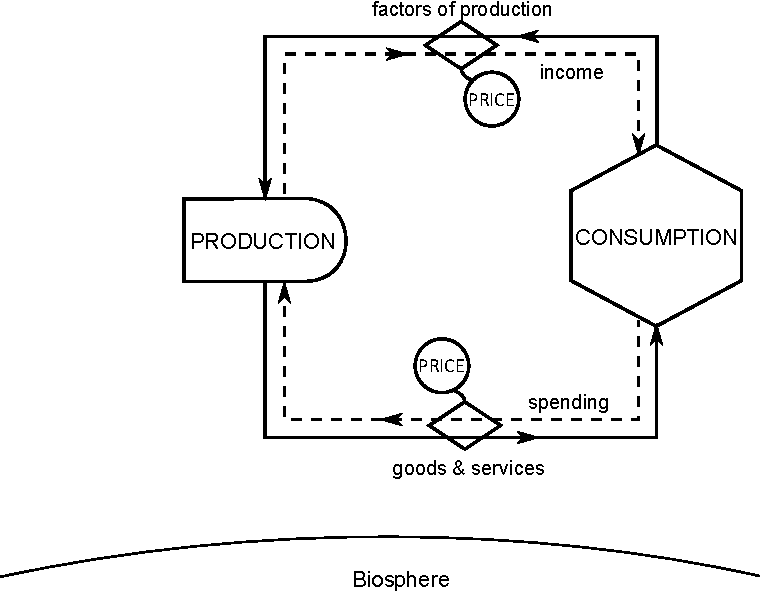
\includegraphics[width=\linewidth]{Part_0/Chapter_Introduction/images/Perpetual_motion_1.pdf}
\caption[The traditional economic model of the economy]{The economy 
is represented as a circular flow of goods and services between two sectors. 
The producers manufacture goods and services 
by taking in labor and capital. 
Consumers exchange labor for wages 
which are used to purchase 
the goods and services of the producers.}
\label{fig:perp_motion_1}
\end{figure}

The traditional model of the economy depicted in Figure~\ref{fig:perp_motion_1} 
is informed by the ``isolated machine metaphor.''
The isolated machine metaphor is an example, as discussed above, 
of a simplification that helps us make sense of the world around us.
Metaphors inform our thinking about the real world,
but consequently,
they also constrain our ability to frame reality.
We mistake the model-metaphor for reality, and
we interact with reality in the same manner 
as we interact with the abstract objects of our
models.\footnote{This fallacious process is called
	\emph{reification}; the making (\emph{facere}, Latin) real of
	something (\emph{res}, Latin) that is merely an idea.
	Alfred Whitehead refers to this as
	\emph{the fallacy of misplaced concreteness}.\cite{Whitehead2011}}
Classical physics told us the universe is
\emph{like} clockwork, 
so we began to interact with the universe
as if it \emph{really were} clockwork.
It then became easy to collect data that confirmed the clockwork model,
because the model told us which data to collect.

The isolated machine metaphor and the traditional model of the economy
preclude any sort of connection 
between the economy and the biosphere.
Thus, only the internal dynamics of the economy are important. 
They tells us that natural resources are unimportant, effectively assuming 
that the biosphere will always provide.
If a particular resource becomes scarce, 
substitution to a different, more-readily-available resource will be made.
They tells us that wastes are unimportant, effectively assuming that the biosphere
has infinite assimilative capacity.
Finally, the isolated machine metaphor and traditional model of the economy 
tell us that economic forces 
(through prices and the market mechanism) will smoothly guide any transition
to good and just outcomes.
In short, the machine can and will carry on.

**** MCD - it seems strange to me to only have one subsection for this section. 
I've split the existing stuff about a need for a new metaphor into a subsection
and added the other subsections below using content from the previous version.
Not sure this is the right place for them.
****

%%%%%%%%%% Resource metaphors %%%%%%%%%%
\subsection{The mechanical metaphor}
\label{sec:mechanical_metaphor}
%%%%%%%%%% 

Thermodynamics tells us that all physical processes require
a transfer of energy.
Because Figure~\ref{fig:perp_motion_1} has no flow of energy
to the economy,
we may consider it a perpetual motion machine
of the \emph{first kind}:
it produces work without the input of energy and
thus violates the First Law of Thermodynamics---the 
law of conservation of energy.\cite{Rao2004}
%The real circulatory system is connected to the lungs,
%from where it takes in oxygen,
%and to the digestive system, 
%where it takes in processed food,
%which are passed to the cells throughout the body.
%This is a major function of the blood:
%to act as an intermediary between the input of energy
%and material resources,
%the food we eat and air we breathe,
%and the internal working of the body.
%The circulatory system is necessarily connected 
%to its environment and circulates energy and materials
%that have been extracted from it.

The economy as an isolated system
represents a ``perpetual motion machine,'' % chktex 38
seemingly able to operate indefinitely with 
no binding constraints.
Because these physical elements of the biosphere are absent from economic models,
the physical constraint they place on the allocation of resources, distribution of outputs, and 
scale of an economy are outside the scope of neoclassical economic discussion.~\cite{Daly1995}

%Current economic models assume
%continued economic growth is possible, 
%necessary, and good. Thus, questions about
%the appropriate scale for the economy 
%are not asked. Even if they were, those questions
%could not be answered because the
%required data are not collected. 
%As the population of the world grows, will we 
%be able to create enough cars to satisfy the growing demand?
%Can we meet the increasing demand for steel, rubber, glass,
%and fuel without considering the consequences? 
%Will there be enough energy to power the 
%automobile factories as 
%well as the increasing number of cars? Will the 
%environment be able to assimilate an ever-increasing 
%amount of pollution?
%
%The mainstream response to those questions
%has been to assume that over a long enough
%time period, economies are not bound by physical 
%limits because of \emph{factor substitutability}.
%A particular energy resource (oil) may be in short supply,
%but our technological expertise---which expands
%as the economy grows---will allow us to substitute
%another resource (coal) for it.
%Substitution may continue indefinitely thus, so
%goes the story,
%the only limiting resource is
%human ingenuity.\cite{Simon1981, Simon1998}
%
%This assumption was thrown into stark relief following the oil
%shocks of the Seventies.
%Suddenly the global economy was thrown
%into reverse for lack of one fundamental resource.
%The necessity of including,
%at the very least,
%energy resources into the economic picture
%spurred the efforts of early (net) energy 
%analysts.\cite{Gilliland1975, Chapman1976}

Figure~\ref{fig:perp_motion_2} depicts the traditional
economic model updated to account for 
energy flows from the biosphere
into the economy.
The economy has changed from an \emph{isolated}
system into an \emph{closed} system,
since only energy inputs have been accounted.

The metaphor for such a model is still very much
a mechanistic one.
The economy is perceived as a machine or engine which,
much like the engines of the Industrial Revolution,
were well-behaved and amenable to control.
Machine metaphors abound in our economic discussions.
We speak of the ``fueling'' the ``economic engine'' 
lest it should ``stall.''~\cite{Liu2012}
Like a well-running engine, the economy is assumed 
to be resilient to small and even quite large perturbations.  
It can either self-correct, 
or be corrected with adjustments to
a few predictable policy levers. 
Additionally, the biosphere is relegated to the position
of a provider of resources;
the larder of the economy.\cite{Norgaard2010}

\begin{figure}[!ht]
\centering\
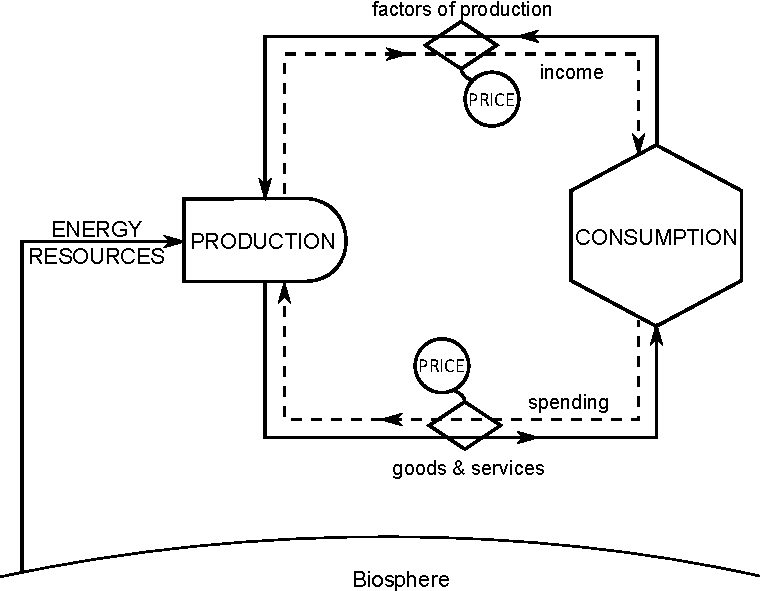
\includegraphics[width=\linewidth]{Part_0/Chapter_Introduction/images/Perpetual_motion_2.pdf}
\caption[The traditional model supplemented with energy inputs]{Energy input output 
analysis has included the flows into the economy from the environment.
This may be considered a perpetual motion machine 
of the second kind.}
\label{fig:perp_motion_2}
\end{figure}

****

%%%%%%%%%% A new metaphor %%%%%%%%%%
\subsection{A new metaphor}
\label{sec:new_metaphor}
%%%%%%%%%% 

When our collective imagination is stuck on a metaphor that 
informs models in which the economy is isolated from the biosphere,
the suggestion to ``account for the environment'' is unconvincing, and 
the challenges cited earlier (natural resource extraction limits,
difficulty of material and energy substitutions, and 
exceeding the biosphere's waste assimilation capacity)
seem unimportant. 

But, mounting evidence shows otherwise. 
Thus, we need to find a new way to understand the complex, 
messy dynamics of real-world economies,
we need a new way to make sense of real-world events, 
we need a new way to learn where and how economies can go wrong, and
we need to plan for the impending materials and energy transformations.
To do so, we had better be counting data that informs \emph{dynamic} models
guided by metaphors that tell us \emph{more} than ``the world is an orderly place.''
Our counting needs to be informed by metaphors and models that are
able to cope with rapid transience,
not just ordered stability.

We need a new metaphor.



%%%%%%%%%% An Apt Metaphor %%%%%%%%%%
\section{An apt metaphor for the economy}
\label{sec:apt_metaphor}
%%%%%%%%%%

If the isolated and machine metaphors are unsuitable, 
what might an apt metaphor for the economy be?
And, if we find an apt metaphor, what types of models would it inform?
Furthermore, what data would the models tell us to collect?
That is, how should we account for the environment?

To begin the search for an apt metaphor, 
we might first ask the question, 
what characteristics are required of an apt metaphor for the economy?
In our opinion, an apt metaphor should account for the fact 
that a real economy:

\begin{enumerate}
	\item{intakes material and energy from the biosphere,}
	\item{exchanges materials and information internally,}
	\item{discharges wastes to the biosphere,}
	\item{is affected by energetic costs,}
	\item{is affected non-linearly by scarcity in the face of low substitutibility,}
	\item{can change in discrete, non-linear fashion with the potential 
			for structural transformation, and}
	\item{embodies energy in material stocks.}
	\item{maintains organizational structure despite changes in the environment\footnote{We note that 
			several areas of the literature speak to the items in this list.
			Material Flow Analysis (MFA) and 
			Economy-Wide Material Flow Analys (EW-MFA)
			stress the importance of
			material intake by the economy. 
			(See Section~\ref{sec:materials_auto}.)
			The Input-Output (I-O) method highlights the effects of internal exchanges
			of material and information with economies. 
			(See Chapter~\ref{chap:intensity}.)
			Life-Cycle Assessment (LCA) techniques focus attention 
			on otherwise-neglected wastes. 
			(See Section~\ref{sec:intensity_auto}.)
			Net Energy Analysis (NEA) predicts that energy resource 
			scarcity reduces Energy Return on Investment (EROI)
			and increases energy prices.
			(See Sections~\ref{sec:B_energy} 
			and~\ref{sec:resource_quality_and_irreversibility}.)
			The Energy Input-Output (EI-O) method gives prominence to energetic costs
			for internal material and energy flows.
			(See Chapter~\ref{chap:intensity}.)
			And, thermodynamic control-volume modeling describes
			transient behavior and system transformations.
			(See Chapters~\ref{chap:materials}--\ref{chap:value}.)
			However, MFA, EW-MFA, I-O, EI-O, LCA, and NEA create snapshots 
			of flows within economies. 
			None of the techniques above (except thermodynamic control-volume modeling) 
			provides structural information. 
			In other words, most of these methods talk about blood, not bones. 
			We contend later (see Section~\ref{sec:apt_models}) that both flows (blood) 
			and structure (stocks, bones) need to be understood.
			Thermodynamic control-volume modeling provides the capability 
			to understand both flows and stocks.}}
\end{enumerate}

Living metabolisms\footnote{The 
	Greek root of metabolism 
	(\emph{metabol$\bar{e}$}) means ``change.''}
exhibit the characteristics in the list above.
Metabolisms and the organisms they support
are intimately connected with the biosphere:
they withdraw materials and energy from the biosphere~(1), 
transfer materials and energy internally via metabolic processes~(2), 
and discharge wastes back to the biosphere~(3).
Metabolisms are affected by energetic costs~(4): 
an organism that obtains less energy than it expends is doomed.
Metabolisms exist in a state of dynamic stability~(5),
adjusting and readjusting to maintain their internal conditions
despite changes in the environment; 
for a metabolism, equilibrium means death!
Metabolisms enable non-linear structural transformations
in their host organisms (e.g., metamorphosis, puberty, and evolution)~(6).
And, energy absorbed into a metabolism is considered to be ``embodied''
in the cells of the organism~(7).

**** Can we include another picture here? 
The one with energy and waste flows out of the economy? MKH.
****

The economy is society's metabolism.\cite{F-K1998, Giampietro2000, Giampietro2013}


%%%%%%%%%% Apt Models %%%%%%%%%%
\section{An apt material, energy, and economy model}
\label{sec:apt_models}
%%%%%%%%%%

As discussed in Section~\ref{sec:metaphors_and_models}, 
metaphors give rise to models.
So, a natural question is: 
``what types of models does the metabolism metaphor inform?''

%%% BRH says that this sentence seems awkward and unnecessary
%%%  But, before developing our models, we again inquire about attributes:
%%% ``what attributes should be present in models informed
%%% by the metabolism metaphor?''
In our opinion, apt models should have the following characteristics:

\begin{enumerate}
	\item{account for flows of materials and energy into, within, and out of the economy,}
	\item{account for accumulation of materials and energy within the economy,}
	\item{provide metrics that relate energy demands and economic value, and}
	\item{provide results that are comparable against existing 
			(or expanded) systems of national accounts.}
\end{enumerate}

Transient conservation equations, often employed by thermodynamicists, 
can account for both flows~(1) and accumulation~(2) of materials
and energy within systems.
We will adapt an existing energy analysis method to develop a 
technique for obtaining metrics of energy and economic value~(3).
Finally, we note that systems of national accounts use the economic sector
as their level of analysis. 
Thus, our models should be also implemented at the economic sector level
so that results from the models we develop can be 
compared against existing (or expanded) systems of national accounts~(4).


%%%%%%%%%% What to Count %%%%%%%%%%
\section{What to count?}
\label{sec:what_to_count}
%%%%%%%%%%

We contend that society is not accounting materials and energy adequately 
in order to plan for the coming material and energy transformations.
After settling on the metabolism metaphor for the economy, 
and after deciding to employ transient thermodynamic equations to develop our model, 
are we any further ahead?
More importantly, will this model allow consumers, producers,
and policy-makers to answer critical questions that are not
answerable today? 
We think so, as we shall endeavor to demonstrate in the remainder of this book.
We believe the key to understanding how energy transformations will unfold
involves specifically understanding how

\begin{itemize}
	\item{materials,}
	\item{energy,}
	\item{embodied energy, and}
	\item{economic value}
\end{itemize}

\noindent{}each flow and accumulate within society's metabolism, the economy.
Of course, each of the above items interacts with the others 
and the biosphere dynamically.
If we can begin to carefully track these items, 
we will be on our way to gathering the information required to 
assist planning for upcoming materials and energy transformations.

To summarize Sections~\ref{sec:apt_metaphor}--\ref{sec:what_to_count}, 
our approach is to:

****MCD - not sure which is preferable **** 
 
\begin{quote}
\begin{normalsize}
develop a dynamic model 
by applying rigorous thermodynamics 
to materials and energy flows into, among, and out of economic sectors,
informed by the metabolism metaphor,
in a manner that is verifiable against 
the existing (or expanded) System of National Accounts (SNA).
\end{normalsize}
\end{quote}

\noindent{}\fbox{\parbox[b][][t]{\textwidth}{\begin{quote}
\begin{normalsize}
develop a dynamic model 
by applying rigorous thermodynamics 
to materials and energy flows into, among, and out of economic sectors,
informed by the metabolism metaphor,
in a manner that is verifiable against 
the existing (or expanded) System of National Accounts (SNA).
\end{normalsize}
\end{quote}}}

****

\noindent{}If successful, we will have developed a framework 
that accounts for the environment. 


%%%%%%%%%% Structure %%%%%%%%%%
\section{Structure of the book}
\label{sec:structure}
%%%%%%%%%%

The list in Section~\ref{sec:what_to_count} 
provides the beginning of the structure for the rest of this book.

Part~\ref{part:matter} addresses flows of physical matter and energy
through the economy.
Chapter~\ref{chap:materials} discusses material flows and accumulation.
Flows of energy are covered in Chapter~\ref{chap:direct_energy}, 
and a rigorous, thermodynamics-based definition of and accounting for 
embodied energy is presented in Chapter~\ref{chap:embodied_energy}.
Throughout the methodological chapters~(\ref{chap:materials}--\ref{chap:value}),
our accounting framework is developed
through a series of increasingly-disaggregated
models of the economy~(Table~\ref{tab:examplesABC}).

In Part~\ref{part:values} we turn to flow and accumulation of 
non-physical entities through the economy. 
Flows and accumulation of economic value are discussed in Chapter~\ref{chap:value}.
In Chapter~\ref{chap:intensity} we combine the results from 
Chapters~\ref{chap:embodied_energy} and~\ref{chap:value} to
calculate an important indicator of economic activity:
the energy intensity of economic production.

Part~\ref{part:implications} gives context to the framework developed in
Parts~\ref{part:matter}~and~\ref{part:values}.
Chapter~\ref{chap:implications} draws out some of the direct implications
of our framework.
Chapter~\ref{chap:unfinished_business} looks at 
unfinished business: practical, conceptual, and theoretical issues
that arise in the development of this framework.
And, we end with a summary in Chapter~\ref{chap:summary}.



\begin{table}
\caption[Examples used throughout this book]{Examples
used throughout this book.}
\begin{center}
  \begin{tabular}{r @{\hspace{2em}} c @{\hspace{2em}} c @{\hspace{2em}} c @{\hspace{2em}} c}
    \toprule
    Example & Sector 0 & Sector 1 & Sector 2 & Sector 3 \\ 
	\midrule
    A & Biosphere	&	Society            & NA         & NA                 \\
    B & Biosphere	&	Final Consumption  & Production & NA                 \\
    C & Biosphere	&	Final Consumption  & Energy     & Goods \& Services  \\
  \bottomrule
  \end{tabular}
\end{center}
\label{tab:examplesABC}
\end{table}
 
Throughout the book, we use the U.S. auto industry 
as a running example for application and discussion.
%
%**** Add more detail to justify the auto industry example. **** 
%
%**** Here are notes from previous email corresondence. ****
%
The running example of the US auto industry demonstrates that our dynamic model 
can be tied to the System of National Accounts, 
thereby meeting one of the requirements for a dynamic model. 
%Our purpose is not to update previous energy intensity calculations.
%
The US auto industry example shows where data are available 
(e.g., economic value, Chapter~\ref{chap:value}), 
where it is old (e.g., energy intensity, Chapter~\ref{chap:intensity}), 
and where it has never been available 
(e.g., accumulated embodied energy, Chapter~\ref{chap:embodied_energy}).  
The US auto industry is, therefore, 
illustrative of the challenges inherent in obtaining data that would feed the model.
%
%**** The following notes are from the authors telecon on Tue 15 Apr 2014. ****
%
%Historical: Berry and Fels
%
%Economic importance
%
%Social/cultural importance
%
%Large energy consumer (both directly and indirectly)
%
%**** The next paragraph is the original paragraph about the auto industry 
%from v1 of the Introduction. ****

The auto industry has been used previously
in the literature in both 
process-based~\cite{Berry:1973vo, Sullivan1995, Stodolsky1995, 
							Sullivan1998, McCleese2002, Sullivan2010, Hawkins2012}
and Input-Output~\cite{Bullard:1978vd, MacLean1998, MacLean2003}
analysis methods,
Furthermore, the industry
remains a large portion of many industrialized economies, 
is very resource intensive, 
has obvious links with energy because
its health is sensitive to disruptions in energy supplies, and
the industry also shows evidence of 
post-industrial decline (shrinking profit margins, etc.).

\bibliographystyle{unsrt}
\bibliography{../../Metabolic}


% Always give a unique label
% and use \ref{<label>} for cross-references
% and \cite{<label>} for bibliographic references
% use \sectionmark{}
% to alter or adjust the section heading in the running head
%% Instead of simply listing headings of different levels we recommend to let every heading be followed by at least a short passage of text. Furtheron please use the \LaTeX\ automatism for all your cross-references and citations.

%% Please note that the first line of text that follows a heading is not indented, whereas the first lines of all sequent paragraphs are.

%% Use the standard \verb|equation| environment to typeset your equations, e.g.
%
%% \begin{equation}
%% a \times b = c\;,
%% \end{equation}
%
%% however, for multiline equations we recommend to use the \verb|eqnarray|
%% environment\footnote{In physics texts please activate the class option \texttt{vecphys} to depict your vectors in \textbf{\itshape boldface-italic} type - as is customary for a wide range of physical jects.}.
%% \begin{eqnarray}
%% a \times b = c \nonumber\\
%% \vec{a} \cdot \vec{b}=\vec{c}
%% \label{eq:01}
%% \end{eqnarray}

%% \section{section Heading}
%% \label{sec:2}
%% Instead of simply listing headings of different levels we recommend to let every heading be followed by at least a short passage of text. Furtheron please use the \LaTeX\ automatism for all your cross-references\index{cross-references} and citations\index{citations} as has already been described in Sect.~\ref{sec:2}.

%% \begin{quotation}
%% Please do not use quotation marks when quoting texts! Simply use the \verb|quotation| environment -- it will automatically render Springer's preferred layout.
%% \end{quotation}


%% \section{section Heading}
%% Instead of simply listing headings of different levels we recommend to let every heading be followed by at least a short passage of text. Furtheron please use the \LaTeX\ automatism for all your cross-references and citations as has already been described in Sect.~\ref{sec:2}, see also Fig.~\ref{fig:1}\footnote{If you copy text passages, figures, or tables from other works, you must obtain \textit{permission} from the copyright holder (usually the original publisher). Please enclose the signed permission with the manucript. The sources\index{permission to print} must be acknowledged either in the captions, as footnotes or in a separate section of the book.}

%% Please note that the first line of text that follows a heading is not indented, whereas the first lines of all sequent paragraphs are.

% For figures use
%
%% \begin{figure}[b]
%% \sidecaption
% Use the relevant command for your figure-insertion program
% to insert the figure file.
% For example, with the option graphics use
%% \includegraphics[scale=.65]{figure}
%
% If not, use
%\picplace{5cm}{2cm} % Give the correct figure height and width in cm
%
%% \caption{If the width of the figure is less than 7.8 cm use the \texttt{sidecapion} command to flush the caption on the left side of the page. If the figure is positioned at the top of the page, align the sidecaption with the top of the figure -- to achieve this you simply need to use the optional argument \texttt{[t]} with the \texttt{sidecaption} command}
%% \label{fig:1}       % Give a unique label
%% \end{figure}


%% \paragraph{Paragraph Heading} %
%% Instead of simply listing headings of different levels we recommend to let every heading be followed by at least a short passage of text. Furtheron please use the \LaTeX\ automatism for all your cross-references and citations as has already been described in Sect.~\ref{sec:2}.

%% Please note that the first line of text that follows a heading is not indented, whereas the first lines of all sequent paragraphs are.

%% For typesetting numbered lists we recommend to use the \verb|enumerate| environment -- it will automatically render Springer's preferred layout.

%% \begin{enumerate}
%% \item{Livelihood and survival mobility are oftentimes coutcomes of uneven socioeconomic development.}
%% \begin{enumerate}
%% \item{Livelihood and survival mobility are oftentimes coutcomes of uneven socioeconomic development.}
%% \item{Livelihood and survival mobility are oftentimes coutcomes of uneven socioeconomic development.}
%% \end{enumerate}
%% \item{Livelihood and survival mobility are oftentimes coutcomes of uneven socioeconomic development.}
%% \end{enumerate}


%% \paragraph{paragraph Heading} In order to avoid simply listing headings of different levels we recommend to let every heading be followed by at least a short passage of text. Use the \LaTeX\ automatism for all your cross-references and citations as has already been described in Sect.~\ref{sec:2}, see also Fig.~\ref{fig:2}.

%% Please note that the first line of text that follows a heading is not indented, whereas the first lines of all sequent paragraphs are.

%% For unnumbered list we recommend to use the \verb|itemize| environment -- it will automatically render Springer's preferred layout.

%% \begin{itemize}
%% \item{Livelihood and survival mobility are oftentimes coutcomes of uneven socioeconomic development, cf. Table~\ref{tab:1}.}
%% \begin{itemize}
%% \item{Livelihood and survival mobility are oftentimes coutcomes of uneven socioeconomic development.}
%% \item{Livelihood and survival mobility are oftentimes coutcomes of uneven socioeconomic development.}
%% \end{itemize}
%% \item{Livelihood and survival mobility are oftentimes coutcomes of uneven socioeconomic development.}
%% \end{itemize}

%% \begin{figure}[t]
%% \sidecaption[t]
% Use the relevant command for your figure-insertion program
% to insert the figure file.
% For example, with the option graphics use
%% \includegraphics[scale=.65]{figure}
%
% If not, use
%\picplace{5cm}{2cm} % Give the correct figure height and width in cm
%
%% \caption{Please write your figure caption here}
%% \label{fig:2}       % Give a unique label
%% \end{figure}

%% \runinhead{Run-in Heading Boldface Version} Use the \LaTeX\ automatism for all your cross-references and citations as has already been described in Sect.~\ref{sec:2}.

%% \runinhead{Run-in Heading Italic Version} Use the \LaTeX\ automatism for all your cross-refer\-ences and citations as has already been described in Sect.~\ref{sec:2}\index{paragraph}.
% Use the \index{} command to code your index words
%
% For tables use
%
%% \begin{table}
%% \caption{Please write your table caption here}
%% \label{tab:1}       % Give a unique label
%
% For LaTeX tables use
%
%% \begin{tabular}{p{2cm}p{2.4cm}p{2cm}p{4.9cm}}
%% \hline\noalign{\smallskip}
%% Classes & class & Length & Action Mechanism  \\
%% \noalign{\smallskip}\svhline\noalign{\smallskip}
%% Translation & mRNA$^a$  & 22 (19--25) & Translation repression, mRNA cleavage\\
%% Translation & mRNA cleavage & 21 & mRNA cleavage\\
%% Translation & mRNA  & 21--22 & mRNA cleavage\\
%%Translation & mRNA  & 24--26 & Histone and DNA Modification\\
%%\noalign{\smallskip}\hline\noalign{\smallskip}
%%\end{tabular}
%%$^a$ Table foot note (with superscript)
%%\end{table}
%
%% \section{Section Heading}
%%\label{sec:3}
% Always give a unique label
% and use \ref{<label>} for cross-references
% and \cite{<label>} for bibliographic references
% use \sectionmark{}
% to alter or adjust the section heading in the running head
%% Instead of simply listing headings of different levels we recommend to let every heading be followed by at least a short passage of text. Furtheron please use the \LaTeX\ automatism for all your cross-references and citations as has already been described in Sect.~\ref{sec:2}.

%% Please note that the first line of text that follows a heading is not indented, whereas the first lines of all sequent paragraphs are.

%%If you want to list definitions or the like we recommend to use the Springer-enhanced \verb|description| environment -- it will automatically render Springer's preferred layout.

%%\begin{description}[Type 1]
%%\item[Type 1]{That addresses central themes pertainng to migration, health, and disease. In Sect.~\ref{sec:1}, Wilson discusses the role of human migration in infectious disease distributions and patterns.}
%%\item[Type 2]{That addresses central themes pertainng to migration, health, and disease. In Sect.~\ref{sec:2}, Wilson discusses the role of human migration in infectious disease distributions and patterns.}
%%\end{description}

%%\section{section Heading} %
%% In order to avoid simply listing headings of different levels we recommend to let every heading be followed by at least a short passage of text. Use the \LaTeX\ automatism for all your cross-references and citations citations as has already been described in Sect.~\ref{sec:2}.

%% Please note that the first line of text that follows a heading is not indented, whereas the first lines of all sequent paragraphs are.

%% \begin{svgraybox}
%% If you want to emphasize complete paragraphs of texts we recommend to use the newly defined Springer class option \verb|graybox| and the newly defined environment \verb|svgraybox|. This will produce a 15 percent screened box 'behind' your text.

%% If you want to emphasize complete paragraphs of texts we recommend to use the newly defined Springer class option and environment \verb|svgraybox|. This will produce a 15 percent screened box 'behind' your text.
%% \end{svgraybox}


%% \section{section Heading}
%%Instead of simply listing headings of different levels we recommend to let every heading be followed by at least a short passage of text. Furtheron please use the \LaTeX\ automatism for all your cross-references and citations as has already been described in Sect.~\ref{sec:2}.

%% Please note that the first line of text that follows a heading is not indented, whereas the first lines of all sequent paragraphs are.

%% \begin{theorem}
%% Theorem text goes here.
%% \end{theorem}
%
% or
%
%% \begin{definition}
%% Definition text goes here.
%% \end{definition}

%% \begin{proof}
%\smartqed
%% Proof text goes here.
%% \qed
%% \end{proof}

%%\paragraph{Paragraph Heading} %
%% Instead of simply listing headings of different levels we recommend to let every heading be followed by at least a short passage of text. Furtheron please use the \LaTeX\ automatism for all your cross-references and citations as has already been described in Sect.~\ref{sec:2}.

%% Note that the first line of text that follows a heading is not indented, whereas the first lines of all subsequent paragraphs are.
%
% For built-in environments use
%
%%\begin{theorem}
%%Theorem text goes here.
%%\end{theorem}
%
%%\begin{definition}
%%Definition text goes here.
%%\end{definition}
%
%%\begin{proof}
%%\smartqed
%% Proof text goes here.
%%\qed
%%\end{proof}
%
%% \begin{acknowledgement}
%% If you want to include acknowledgments of assistance and the like at the end of an individual chapter please use the \verb|acknowledgement| environment -- it will automatically render Springer's preferred layout.
%% \end{acknowledgement}
%
%% \section*{Appendix}
%% \addcontentsline{toc}{section}{Appendix}
%
%% When placed at the end of a chapter or contribution (as opposed to at the end of the book), the numbering of tables, figures, and equations in the appendix section continues on from that in the main text. Hence please \textit{do not} use the \verb|appendix| command when writing an appendix at the end of your chapter or contribution. If there is only one the appendix is designated ``Appendix'', or ``Appendix 1'', or ``Appendix 2'', etc. if there is more than one.

%% \begin{equation}
%% a \times b = c
%% \end{equation}
% Problems or Exercises should be sorted chapterwise
%% \section*{Problems}
%% \addcontentsline{toc}{section}{Problems}
%
% Use the following environment.
% Don't forget to label each problem;
% the label is needed for the solutions' environment
%% \begin{prob}
%% \label{prob1}
%% A given problem or Excercise is described here. The
%% problem is described here. The problem is described here.
%% \end{prob}

%% \begin{prob}
%% \label{prob2}
%% \textbf{Problem Heading}\\
%% (a) The first part of the problem is described here.\\
%% (b) The second part of the problem is described here.
%% \end{prob}


